\documentclass[12pt]{article}

\usepackage{sbc-template}

\usepackage{graphicx,url}

\usepackage[brazil]{babel}   
%\usepackage[latin1]{inputenc}  
% UTF-8 encoding is recommended by ShareLaTex
\usepackage[utf8]{inputenc}
\usepackage{listings}

\widowpenalty=10000


\clubpenalty=10000

\usepackage{color}
\usepackage{float}

\definecolor{codegreen}{rgb}{0,0.6,0}
\definecolor{codegray}{rgb}{0.5,0.5,0.5}
\definecolor{codepurple}{rgb}{0.58,0,0.82}
\definecolor{backcolour}{rgb}{0.95,0.95,0.92}
 
\lstdefinestyle{mystyle}{
    backgroundcolor=\color{backcolour},   
    commentstyle=\color{codegreen},
    keywordstyle=\color{magenta},
    numberstyle=\tiny\color{codegray},
    stringstyle=\color{codepurple},
    basicstyle=\footnotesize,
    breakatwhitespace=false,         
    breaklines=true,                 
    captionpos=b,                    
    keepspaces=true,                 
    numbers=left,                    
    numbersep=5pt,                  
    showspaces=false,                
    showstringspaces=false,
    showtabs=false,                  
    tabsize=2
}
 
\lstset{style=mystyle}
\renewcommand{\lstlistingname}{Quadro}

\sloppy

\title{Aceleração de uma Aplicação Científica com OpenCL: Regularização de Dados Sísmicos}

\author{Vanderson Martins do Rosario\inst{1}}


\address{Instituto de Computação -- Universidade Estadual de Campinas (Unicamp)\\
  Campinas -- SP -- Brasil
}

\begin{document} 

\maketitle
     
\begin{resumo} 
Este trabalho apresenta uma sequência de transformações aplicadas sobre um código, inicialmente sequêncial, para que esse obtenha o máximo desempenho sobre um processador \textit{multicore} e uma placa de vídeo por meio do \textit{framework} OpenCL. Durante o desenvolvimento do trabalho, diversos experimentos foram realizados para medir a eficiência de cada implementação e de cada transformação, tanto para guiá-las quanto para mostrar os impactos das mesmas. Nessa seção, apresentamos a lista dos materias utilizados e as técnicas utilizadas para realização e medição dos experimentos.
\end{resumo}


\section{Introdução}
Este trabalho apresenta uma sequência de transformações aplicadas sobre um código, inicialmente sequêncial, para que esse obtenha o máximo desempenho sobre um processador \textit{multicore} e uma placa de vídeo por meio do \textit{framework} OpenCL. Durante o desenvolvimento do trabalho, diversos experimentos foram realizados para medir a eficiência de cada implementação e de cada transformação, tanto para guiá-las quanto para mostrar os impactos das mesmas. Nessa seção, apresentamos a lista dos materias utilizados e as técnicas utilizadas para realização e medição dos experimentos.

Este trabalho apresenta uma sequência de transformações aplicadas sobre um código, inicialmente sequêncial, para que esse obtenha o máximo desempenho sobre um processador \textit{multicore} e uma placa de vídeo por meio do \textit{framework} OpenCL. Durante o desenvolvimento do trabalho, diversos experimentos foram realizados para medir a eficiência de cada implementação e de cada transformação, tanto para guiá-las quanto para mostrar os impactos das mesmas. Nessa seção, apresentamos a lista dos materias utilizados e as técnicas utilizadas para realização e medição dos experimentos.

Este trabalho apresenta uma sequência de transformações aplicadas sobre um código, inicialmente sequêncial, para que esse obtenha o máximo desempenho sobre um processador \textit{multicore} e uma placa de vídeo por meio do \textit{framework} OpenCL. Durante o desenvolvimento do trabalho, diversos experimentos foram realizados para medir a eficiência de cada implementação e de cada transformação, tanto para guiá-las quanto para mostrar os impactos das mesmas. Nessa seção, apresentamos a lista dos materias utilizados e as técnicas utilizadas para realização e medição dos experimentos.

Este trabalho apresenta uma sequência de transformações aplicadas sobre um código, inicialmente sequêncial, para que esse obtenha o máximo desempenho sobre um processador \textit{multicore} e uma placa de vídeo por meio do \textit{framework} OpenCL. Durante o desenvolvimento do trabalho, diversos experimentos foram realizados para medir a eficiência de cada implementação e de cada transformação, tanto para guiá-las quanto para mostrar os impactos das mesmas. Nessa seção, apresentamos a lista dos materias utilizados e as técnicas utilizadas para realização e medição dos experimentos.
\section{Materiais e Métodos}

Este trabalho apresenta uma sequência de transformações aplicadas sobre um código, inicialmente sequêncial, para que esse obtenha o máximo desempenho sobre um processador \textit{multicore} e uma placa de vídeo por meio do \textit{framework} OpenCL.

Durante o desenvolvimento do trabalho, diversos experimentos foram realizados para medir a eficiência de cada implementação e de cada transformação, tanto para guiá-las quanto para mostrar os impactos das mesmas. Nessa seção, apresentamos a lista dos materias utilizados e as técnicas utilizadas para realização e medição dos experimentos.

\subsection{Materiais}

Todos os experimentos foram realizados sobre uma mesma máquina, Dell Optiplex 9020, equipado com um processador Intel(R) Core(TM) i5-4590 CPU @ 3.30GHz com quatro unidades de processamento e uma GPU Intel(R) HD Graphics 4600 com 20 unidades de processamento com frequência máxima de 1150 MHz. Ainda, a máquina é equipada com 2 pentes de 4GB DDR3 SDRAM de 1600MHz em multiplos canais.

% Precisa da versão do CENTOS 
%TODO
Para compilar o código fonte, foi utilizado o GCC versão 4.8.5 sobre a plataforma CentOS com um \textit{third-party kernel}: 4.4.13\-1.el7.elrepo.x86\_64. Entre os frameworks utilizados, o OpenMP na versão 3.1 e o OpenCL 1.2 com o driver da Intel na versão 16.4.4.47109.

Para todos os experimentos, o código fonte foi compilado com o comando apresentado no Quadro \ref{comandogcc}.\\
\begin{lstlisting}[language=bash, caption=Comando para compilar o código fonte dos experimentos., label=comandogcc]
$ gcc -O3 --std=c99 reg.c semblance.c su.c -lm -I. -lOpenCL -fopenmp
\end{lstlisting}

%As variáveis de ambiente do sistema .... %TODO


\subsection{Experimentos  e Código Fonte}

Utilizou-se, para obter-se as métricas de execução de todos os experimentos, a ferramenta Perf do Linux com o comando do Quadro \ref{comandoperf}. Para cada experimento, foram repetidas 20 execuções seguidas e feito a média dos valores obtidos, levando-se em consideração a lei dos grandes números. Dessa forma, para todos os gráficos apresentados nesse trabalho é mostrado os valores da média juntamente com o desvio padrão. \\ %TODO citar lei dos grandes números.

\begin{lstlisting}[language=bash, caption=Comando para mensurar as métricas de execução., label=comandoperf]
$ perf stat -B -e cache-references,cache-misses,cycles,instructions,branches,branch-misses,faults,migrations
\end{lstlisting}

Ainda, em todos os gráficos de tempo de execução do trabalho, os tempos de execução são mostrados dividos em duas partes: (1) tempo de inicialização e (2) tempo de execução. Onde, o (1) tempo de inicialização é o tempo necessário para inicialização e configuração do OpenCL, alocação da memória, leitura do código-fonte do \textit{kernel}, leitura do arquivo com os dados de entrada e compilação do \textit{kernel}; e o (2) tempo de execução é o tempo para execução do \textit{kernel} mais o tempo para transferência dos dados de entrada e saída. Para medir esses dois tempos, o código foi instrumentado com a função do Quadro \ref{functime}. \\

\begin{lstlisting}[language=c, caption=Função utilizada para calcular o tempo de execução de trexos de código, label=functime]
#include <sys/time.h>

double mysecond() {
  struct timeval tp;
  gettimeofday(&tp ,NULL);
  return ((double) tp.tv_sec + (double) tp.tv_usec * 1.e-6);
}
\end{lstlisting}

O código fonte apresentado e citado no trabalho pode ser obtido por meio do repositório git hospedado no github.com (\url{https://github.com/vandersonmr/REG}). Todas as etapas apresentadas na Seção \ref{desenvolvimento} podem ser vistas pelo histório de \textit{commits} do repositório. Por exemplo, o código com as transformações citadas na Subseção \ref{multi} pode ser obtido com o comando git do Quadro \ref{comandogit}. \\

\begin{lstlisting}[language=bash, caption=Comando para navegar pelas transformações apresentadas no artigo., label=comandogit]
$ git log --oneline
%TODO
$ git reset --hard %TODO
\end{lstlisting}

\section{Desenvolvimento e Resultados} \label{desenvolvimento}

Dado uma implementação sem muitas otimizações de uma solução sequêncial para a regularização de dados sísmicos\ref{borin}, foram primeiramente testados o desempenho dessa solução per si, em seguida o de uma simples paralelização dessa solução com OpenMP e com a paralelização com OpenCL depois de aplicado um conjunto de otimizações.

Nessa seção, apresentamos uma breve análise do código original, sequêncial (\ref{seq}); da paralelização com OpenMP (\ref{omp}), da paralelização com OpenCL (\ref{ocl}), seguido da explicação das diversas otimizações aplicadas sobre a última e seus impactos no desempenho da mesma.

\subsection{Código Sequêncial} \label{seq}

A implementação sequêncial pode ser dividido em três grandes partes, a saber: 

\begin{itemize}
\item \textbf{Inicialização}: Nessa parte, toda contida no arquivo reg.c, o programa lê os parametros passados para o executável (\ref{param}), lê um arquivo contendo os dados sísmicos (\ref{file}) e em seguida cria e preenche estruturas de dados que seram usados pelo \textit{kernel} (\ref{struct}). 

\begin{lstlisting}[language=c, caption=Leitura dos parametros passados para o executável., label=param]
    float m0 = atof(argv[1]);
    float h0 = atof(argv[2]);
    float t0 = atof(argv[3]);
    float tau = strtof(argv[4], NULL);
    
    float p0[5], p1[5];
    int np[5];
 
    for (i = 0; i < 5; i++) {
        p0[i] = atof(argv[5 + 3*i]);
        p1[i] = atof(argv[5 + 3*i + 1]);
        np[i] = atoi(argv[5 + 3*i + 2]);
    }
\end{lstlisting}

Para cada experimento, foram testados 3 conjuntos de parametros como entrada, a saber:

\begin{itemize}
\item Param1: 
\begin{lstlisting}[language=bash]
"4120 -480 1.124 0.005
-0.1     0.1     20 
-0.00143 0.00057 20 
 7.8e-07 9.8e-07 20 
-1.0e-07 1.0e-07 20 
-1.0e-07 1.0e-07 20"
\end{lstlisting}
\item Param2:
\begin{lstlisting}[language=bash]
"4120 -480 1.94 0.005
-0.00088484  0.00111516 20 
-0.001194    0.000806   20 
 6.4e-07     8.4e-07    20 
 6.0e-10     8.0e-10    20 
 4.61e-08    6.61e-08   20"
\end{lstlisting}
\item Param3:
\begin{lstlisting}[language=bash]
"4120 -480 2.255 0.005
-0.001147   0.000853  20 
-0.001139   0.000861  20 
 4.396e-07  5.396e-07 20 
 3.002e-07  4.102e-07 20 
-2.101e-07  0.101e-07 20"
\end{lstlisting}
\end{itemize}

\begin{lstlisting}[language=c, caption=Leitura do arquivo com os dados sismícos., label=file]
    char *path = argv[20];
    FILE *fp = fopen(path, "r");
	...
    su_trace_t tr;
    vector_t(su_trace_t) traces;
    vector_init(traces);

    while (su_fgettr(fp, &tr)) {
        vector_push(traces, tr);
    }
\end{lstlisting}

\begin{lstlisting}[language=c, caption=Preenchimento da estrtura de dados., label=struct]
   aperture_t ap;
    ap.ap_m = 0;
    ap.ap_h = 0;
    ap.ap_t = tau;
    vector_init(ap.traces);
    for (int i = 0; i < traces.len; i++)
        vector_push(ap.traces, &vector_get(traces, i));
\end{lstlisting}


A inicialização ocupa pouco tempo na execução total do programa. A leitura do arquivo é a parte mais demorada (\ref{file}), principalmente quando o programa é executado pela primeira vez. Se executado em sequência, o arquivo já está em \textit{cache} e o tempo da etapa de inicialização cai drasticamente.
\\
\item \textit{\textbf{Kernel}}: Nessa parte, contida no arquivo reg.c e semblance.c, a função \textit{compute\_max} (\ref{max}) chama a função \textit{semblance\_2d} (kernel) diversas vezes. A função \textit{semblance\_2d} (\ref{semblance}), medido pelo Perf, ocupa 97\% do tempo de exeução do programa, portanto, é o trexo mais quente e mais interessante para ser otimizado. 

\begin{lstlisting}[language=c, caption=Corpo da função \textit{compute\_max}., label=max]
for (int ia = 0; ia < np[0]; ia++) {
 float a = n0[0] + ((float)ia / (float)np[0])*(n1[0]-n0[0]);
 for (int ib = 0; ib < np[1]; ib++) {
   float b = n0[1] + ((float)ib / (float)np[1])*(n1[1]-n0[1]);
   for (int ic = 0; ic < np[2]; ic++) {
     float c = n0[2] + ((float)ic / (float)np[2])*(n1[2]-n0[2]);
     for (int id = 0; id < np[3]; id++) {
       float d = n0[3]+((float)id / (float)np[3])*(n1[3]-n0[3]);
       for (int ie = 0; ie < np[4]; ie++) {
         float e = n0[4]+((float)ie/(float)np[4])*(n1[4]-n0[4]);
         float st;
                       
         float s = semblance_2d(ap,a,b,c,d,e,t0,m0,h0,&st);
	  ...
        }
      }
   }
 }
}
\end{lstlisting}

Nota-se que o kernel possui uma frequência alta de execução por estar sendo chamado diversas vezes dentro da função \textit{compute\_max}. Podemos ver a quantidade de \textit{loops} aninhados, sendo a chamada está no nível mais profundo.

\begin{lstlisting}[language=c, caption=Corpo da função \textit{semblance\_2d}., label=semblance]
    for (int i = 0; i < ap->traces.len; i++) {
        tr = vector_get(ap->traces, i);

        float mx, my, hx, hy;
        su_get_midpoint(tr, &mx, &my);
        su_get_halfoffset(tr, &hx, &hy);

        float t = time_2d(A, B, C, D, E, t0, m0, my, h0, hy);
        int it = (int)(t * idt);

        if (it - tau >= 0 && it + tau < tr->ns) {
            for (int j = 0; j < w; j++) {
                int k = it + j - tau;
                float v = interpol_linear(k, k+1,
                        tr->data[k], tr->data[k+1],
                        t*idt + j - tau);
                num[j] += v;
                den[j] += v*v;
                _stack += v;
            }
            M++;
        } else if (++skip == 2) {
            return 0;
        }
    }
\end{lstlisting}

A função \textit{semblance\_2d} possui dois acessos a dados na memória, o primeiro, na linha 2, acessa os \textit{traces} e o seguindo, dentro do \textit{loop}, acessa \textit{data}. Ambos os acessos são sequênciais, por isso, acredita-se que tenham boa localidade.
\\
\item \textbf{Finalização}: Na última parte, é necessário selecionar entre todos os semblances calculados, o melhor. Esse é o trexo mais rápido na execução do código.

\end{itemize}

Testamos o desempenho do código sequêncial com as otimização O0, O2 e O3 com vetorização, apesar do compilador (gcc-4.8.5) não ter conseguido vetorizar o código. O resultado do desempenho médio para cada sequência de otimização pode ser visto no gráfico da Fígura \ref{fgsequencial}.


\begin{figure}[H]
\centering
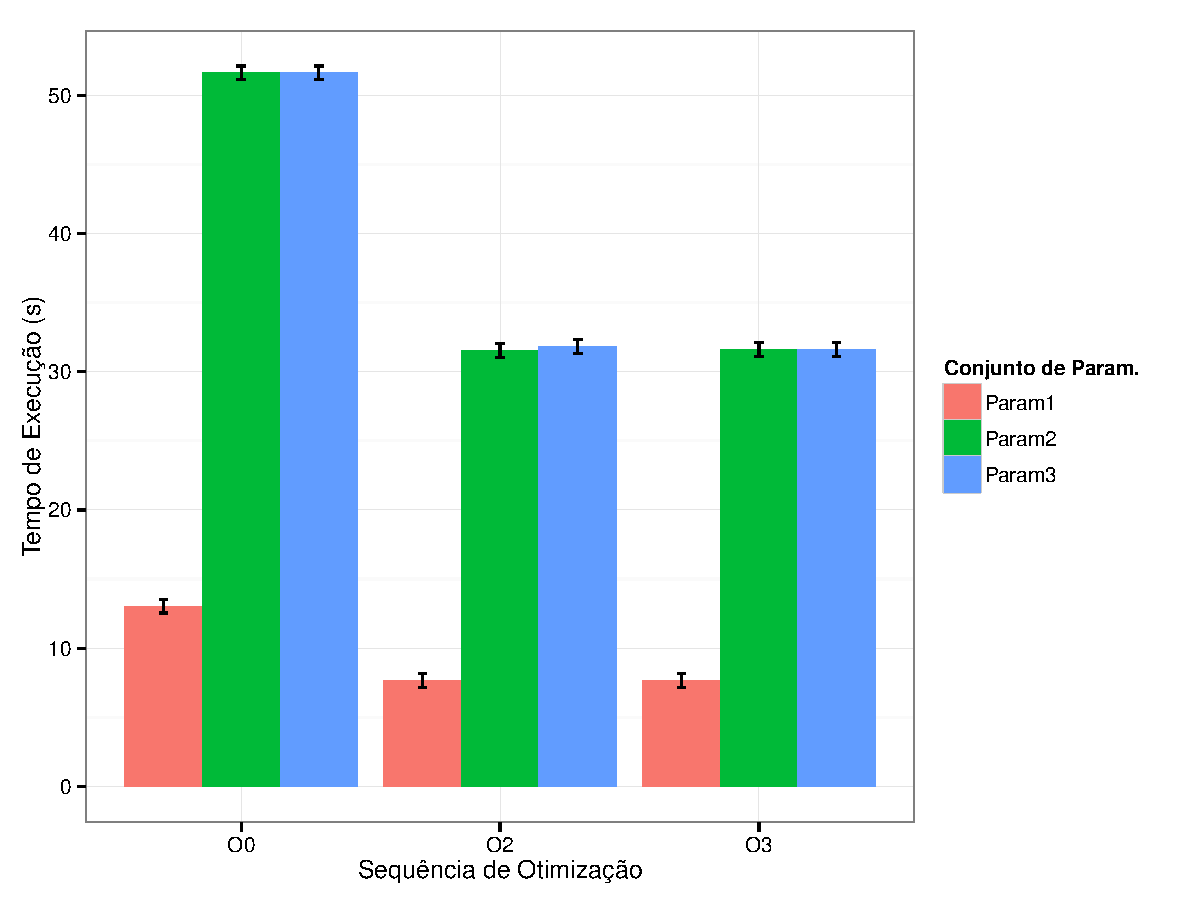
\includegraphics[width=0.8\textwidth]{seq.pdf}
\caption{Tempos de execução do código sequêncial compilado em O0, O2 e O3 para os três conjuntos de parametros de entrada.}
\label{fgsequencial}
\end{figure}

\subsection{Paralelização com OpenMP} \label{omp}

A paralelização utilizando-se do OpenMP foi feita de maneira bem simples: cada iteração do primeiro laço da função \textit{compute\_max} foi lançado em uma thread diferente pelo escalonador do OpenMP. Para isso, o \textit{pragma} do Quadro \ref{openmp} foi adiciona antes da linha do primeiro laço.
\\
\begin{lstlisting}[language=c, caption=\textit{Pragma} para paralelização com OpenMP., label=openmp]
    #pragma omp parallel for schedule(dynamic)
    for (int ia = 0; ia < np[0]; ia++) 
\end{lstlisting}

Além de adicionar o \textit{pragma}, como agora cada \textit{thread} calcula um \textit{semblance}, é preciso manter na memória o resultado de todas as \textit{threads} e depois iterar sobre eles para encontrar o melhor resultado. Com esse objetivo, o código do Quadro \ref{endomp} foi adicionado logo depois que a execução paralela do \textit{kernel} é finalizado. Note-se que foi adicionado diversos vetores que contém os resultados de cada \textit{thread}. \\

\begin{lstlisting}[language=c, caption=Código para selecionar o melhor resultado entre os resultados calculados por cada \textit{thread}., label=endomp]
    float ssmax = -1.0;
    *stack = 0;
    for (int ia = 0; ia < np[0]; ia++) {
        if (smax[ia] > ssmax) {
            *Aopt = _Aopt[ia];
            *Bopt = _Bopt[ia];
            *Copt = _Copt[ia];
            *Dopt = _Dopt[ia];
            *Eopt = _Eopt[ia];
            *stack = _stack[ia];
            *sem = smax[ia];
            ssmax = smax[ia];
        }
    }
\end{lstlisting}

Foram executados os mesmos experimentos da Seção \ref{seq}, mas agora com o código paralelizado para CPU. Obteve-se um \textit{speedup} médio de X como podemos ver na Figura \ref{fgomp}.

\begin{figure}[H]
\centering
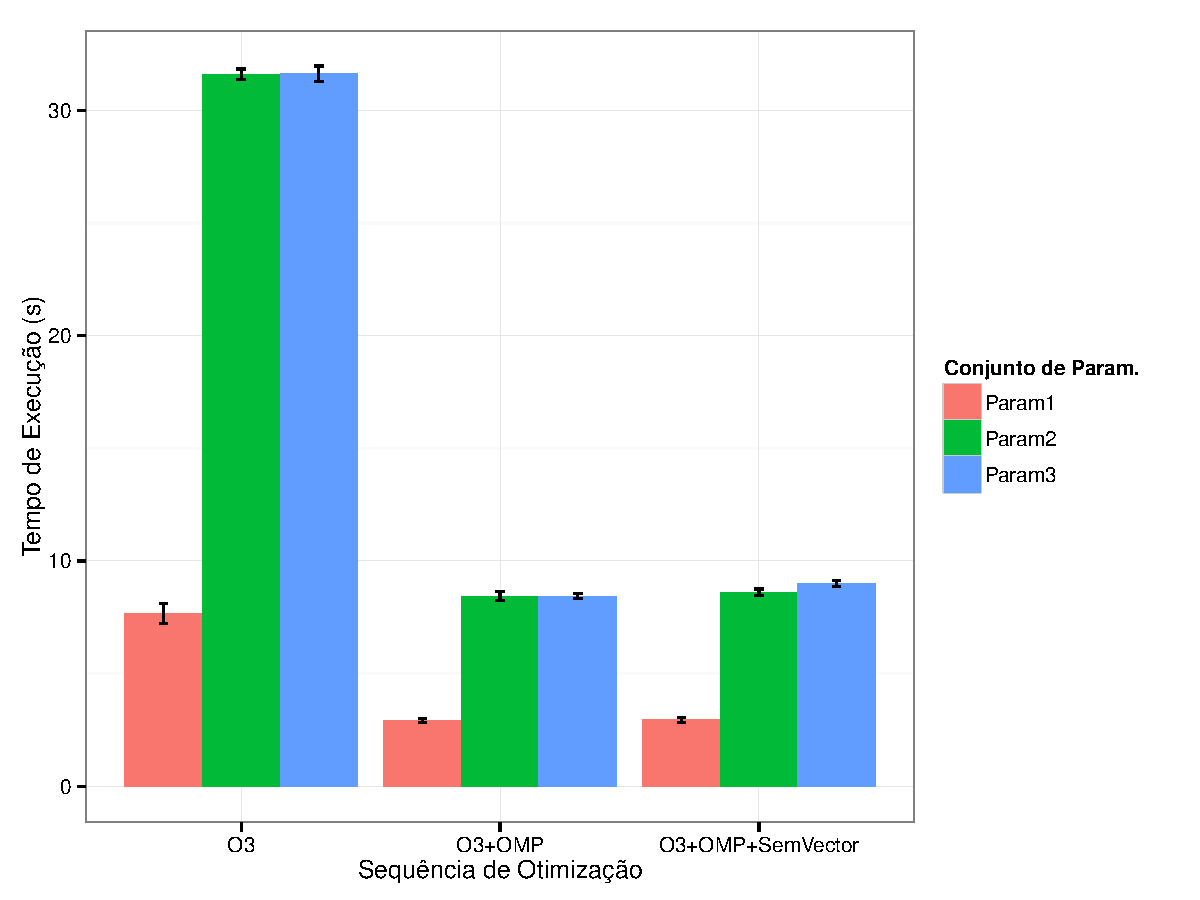
\includegraphics[width=0.8\textwidth]{omp.pdf}
\caption{Tempos de execução do código sequêncial compilado com O3, do código com OpenMP compilado em O3, e do código OpenMP compilado com O3 e sem a estrutura de vetores.}
\label{fgomp}
\end{figure}

O OpenCL permite que o código paralelizado seja executado em diversas arquiteturas, inclusive em GPUs. Isso não é possível com o OpenMP ou com o código original, portanto, as otimizações foram implementadas apenas para o OpenCL. Apesar disso, é possível perceber que a solução com OpenMP poderia se beneficiar das mesmas otimizações e, por isso, não é justo comparar o desempenho das duas implementações. Dessa forma, sabendo que o código OpenMP não pode ser executado nas mesmas plataformas e que não foram aplicadas as mesmas otimizações em sua implementação, o trabalho se concentra em obter o máximo desempenho sobre a implementação em OpenCL, sem se preocupar com comparações com a implementação com OpenMP.

A partir da próxima subseção, todos os resultados mostrados serão de experimentos compilados com O3.

\subsection{Paralelização com OpenCL} \label{ocl}

Falar sobre o OpenCL e como ele funciona.

Falar sobre o que foi necessário para transformar o código do OpenMP para rodar com OpenCL.

Falar sobre CPU bond e Memory Bond e como podemos contornar esses problemas com OpenCL. Falar sobre como fazer vetorização com OpenCL e como a hierarquia de memória funciona. Falar dos manuais.

Instroduzir as otimizações que seram aplicadas.

\subsubsection{Multidimensões} \label{multi}

Falar que diretamente, a GPU ainda não funcionava. 

Falar que ao adicionar mais dimensões houve melhoria no desempenho da CPU e a GPU começou a funcionar. 

Mostrar resultados de desempenho para 2D e 3D.

\subsubsection{Removendo Dados Desnecessários}

Mostrar que no código original grande parte dos dados não estava sendo utilizado. Mostrar como tirar esses dados e como isso manteve a corretude.

Mostrar impacto no desempenho.

\subsubsection{\textit{Inlining} das Funções}

Falar sobre o fato que mesmo os manuais dizendo que o inlining é feito SEMPRE. Vários relatam a mudança de desempenho com inlining manual.

Argumentar que o inlining manual pode criar oportunidade de otimizações manuais que o compilador talvez não consiga fazer.

Mostrar impacto no desempenho.

\subsubsection{Melhor\textit{ Local Work Size}}

Comentar sobre a escolha dos work-local-size.

Falar sobre manual do hardware e clinfo.

Mostrar os melhores valores encontrados.

\subsubsection{Simplificações Algébricas}

Mostrar que os inlinings no kernel permitiram a aplicação de várias simplificações algébricas.

Argumentar que o compilador pode não estar fazendo as simplificações porque os dados são floats, comentar sobre as otimizações (https://www.khronos.org/registry/cl/sdk/1.0/docs/man/xhtml/clBuildProgram.html).

Mostar o impacto no desempenho CPU e GPU.

\subsubsection{\textit{Loop Invariant Code Motion}}

Mostrar como alguns trexos do código são independentes das variáveis de indução e por isso podem ser movidos para fora do loop e até mesmo para fora do kernel.

Mostrar o impacto no desempenho do código.

\subsubsection{\textit{Constant Memory Space}}

Explicar sobre a constant memory space nas GPUs, falar sobre o tamanho dessa memória na GPU da Intel.

Falar quais dados foram escolhidos para ir memória constant.

Mostrar o impacto no desempenho.

\subsubsection{Reduzindo a Pressão Sobre os Registradores }

Falar sobre a hipótese fato que o desempenho do kernel estava sendo limitado por memory bound.

Mas, tirar os acessos diretos a memória não estavam surtindo efeito e eram sequências.

Falar que havia a desconfiança que estava ocorrendo register spill.

Mostrar como os dados foram levados a memória local.

Mostrar o impacto no desempenho.

\subsection{Otimizações Não Implementadas ou Não Mantidas}

Falar sobre o fato que algumas otimizações não foram aplicadas.

\subsubsection{Vetorização}

Falar sobre vetorização no OpenCL e como tentamos aplicar, mas que não houve nenhum benefício.

\subsubsection{Redução}

Falar sobre a posibilidade de fazer alguma espécie de redução, mas que não conseguimos encontrar espaço para essa otimização.

\subsubsection{\textit{Loop Blocking}}

Argumentar que o código não é memory bound e que blocking não seria eficiente.

\section{Problemas Encontrados}

Falar sobre manter corretude sem a alocação;

Falar que não foi escolhido adicionar diversos defines.

Argumentar que muitas das otimizações podem ter diminuido a corretude do código para outras entradas.

\section{Trabalhos Futuros}

Falar sobre analisar o código sobre uma ferramenta sofisticada e investigar se estamos próximos do limite teórico do hardware.

Falar sobre aplicar essas otimizações sobre o OpenMP e medir o desempenho.

Falar sobre as posiveis otimizações que ainda podem ser aplicadas.

\section{Conclusão}

Tentar analisar o desempenho teórico do hardware. Tentar argumentar o desempenho alcançado.

Falar sobre o OpenCL e as otimizações encontradas. Falar sobre os problemas e os trabalhos futuros.

\bibliographystyle{sbc}
\bibliography{sbc-template}

\end{document}
